\documentclass[11pt]{article} % Document type
\title{Assigment 3 \\
    \large Sorting your Affairs in Order\\
     \textbf{WRITEUP.pdf}}
\author{Reuben T. Chavez}
\date{\today} % Sets the date to \today, or any date you specify
\usepackage{graphicx}
\begin{document}
\maketitle % Start the document



\pagebreak

\section*{Synopsis}
The following write-up focuses on the patterns and trends on the various
graphs when running the Collatz program. As well as explain how the
following UNIX commands were able to graph the \textbf{\emph{Collatz Sequence Length}}, \textbf{\emph{
Max Collatz Sequence}}, and \textbf{\emph{ Collatz Sequence Histogram}}. 

\pagebreak
\section*{Collatz Sequence Length Graph}

\begin{figure}[htp]
\centering
\includegraphics[scale=1.00]{length.pdf}
\caption{For n $ \epsilon $ (2 .. 1000)}
\label{Collatz Sequence Length}
\end{figure}

\begin{flushleft}

The Collatz Sequence Length Graph records the length of each Collatz sequence starting at n.
The best way to interpret this notion was to use the UNIX wc -l command, which counts the 
number of characters, words, or lines within a document. Setting up the command was to implement
an iteration where it first appends the x on the .dat file, and then when running the current
number through the Collatz program, the UNIX command | would pipe the results onto the command 
wc -l.

\begin{figure}[htp]
\centering
\includegraphics[scale=.50]{/home/rtchavez/Pictures/length.png}
\caption{}
\label{}
\end{figure}

 It will count the number of lines from the output and append it to the .dat file.
The reason for choosing wc was simple. It was more effective a more straightforward to use the 
command than to implement a nested for loop to find the number of lines within the text.

\end{flushleft}


\pagebreak
\section*{Max Collatz Sequence Graph}
The Max Collatz Sequence Graph records the highest number found within the Collatz sequence of n. 
The process was similar to the last one, where I use an iteration, but mainly different is where 
it's piped after. After using the | command, the output pipes into UNIX's sort and head command 
to find the highest number within each n sequence. 
The idea is that the results will then be 
sorted in numerical order and reversed to have the highest number at the top of the page, 
through sort -r -g, which is then piped to head -n 1 to look for the first line of the output. 
Initially, I had done the opposite, where the highest number would be at the bottom of the page,
and I would use the command tail to look for the last line. However, the coding process would take 
longer. 
Hence the use of sort -r- g and head -n to find the max and then plot it through Gnuplot.

\begin{figure}
\centering
\includegraphics[scale=1.]{max.pdf}
\caption{For n $ \epsilon $ (2 .. 1000)}
\label{}
\end{figure}
\pagebreak

\begin{figure}
\centering
\includegraphics[scale=0.5]{/home/rtchavez/Pictures/max.png}
\caption{}
\label{}
\end{figure}
\pagebreak

\section*{Collatz Sequence Length Histogram}
\begin{figure}[htp]
\centering
\includegraphics[scale=1.00]{histogram.pdf}
\caption{For n $ \epsilon $ (2 .. 1000)}
\label{}
\end{figure}

\begin{flushleft}

The Collatz Sequence Histogram records how frequently a particular length of a Collatz sequence 
can be found after iterating through n. The process used the UNIX wc -l command in an iteration 
and then appended the different lengths to a .dat file. After the iteration, I decided to 
implement three UNIX commands, cat, sort, uniq, and sed, to count the number of repetitions 
within the file and append them to the .dat file.
 
\begin{figure}[htp]
\centering
\includegraphics[scale=.5]{/home/rtchavez/Pictures/histogram.png}
\caption{}
\label{}
\end{figure}

After iterating, the file was called through 
cat to print the contents of the .dat file, so the program could pipe the output to sort -r -g,
 where the program then reorganized the data within the file in reverse and numerical order. This 
process was done so that uniq can count the repeated sequences within the .dat a lot faster and 
eliminates the chance to miss a number. Without the sort command, the program would recount numbers 
without taking notice.
The process for uniq would go a lot faster since the numbers are organized 
instead of searching for every number while going back and forth. With uniq it was set to only 
count the repeated lines with uniq -c -d. After that, it piped to sed. Prior to using sed, it didn't 
plot any of the points because the white space was caused by uniq -c -d, resulting in errors when
 plotting a graph.
\end{flushleft}

\end{document}
\grid

